\label{analise_monitoramento_servicos}

Com realização da implementação, implantação e integração das aplicações para execução do monitoramento,é necessário a divulgação da análise e dos resultados do trabalho executado. Este Capítulo apresenta a análise realizada após a execução do Ems-Monitor.

%%%%%%%%%%%%%%%%%%%%%%%%%%%%%%%%%%%%%%%%%%%%%%%%%%%%%%%%%%%%%%%

\section{Análise das Aplicações}
\label{analise}
Com propósito de avaliar a execução do Ems-Monitor, foram analisados alguns requisitos das plataformas utilizadas para monitorar o Erlangms, por meio de uma ferramenta de monitoramento. Inicialmente os requisitos dos recursos computacionais das aplicações foram avaliados, tanto o requisito do barramento de serviços quanto o da ferramenta de monitoramento. 

O agente de monitoramento utiliza os mesmos recuros computacionais do \textit{software} onde ele foi implantado, nesse caso o agente de monitoramento é representado pelo \textit{software} Exometer e está implantado no barramento de serviços Erlangms, os requisitos de instalação do barramento de serviços poderão ser visualizados em \cite{erlangms_gitHub}, assim como os requisitos de configuração do Exometer poderão ser visualizados em \cite{exometer_gitHub}. A ferramenta de monitoramento também dispõe de requisitos básicos para seu funcionamento, os requisitos do Nagios Core\textsuperscript{\textregistered} na versão quatro poderão ser visualizados em \cite{nagios_core_configuration}, em ambos os caso os requisitos computacionais não impediram a execução do projeto e consequentemente foram executados sem gerar grandes esforços.

Dispondo da configuração das aplicações foi necessário realizar a avaliação do funcionamento do monitoramento, por meio do conjunto de protocolos TCP/IP, onde sabe-se que o protocolo \acrshort{SNMP} é um protocolo da \textit{Internet}, que por sua vez o protocolo \acrshort{SNMP} para garantir a transmissão dos dados de monitoramento utilizada por padrão o protocolo UDP especificamente nas portas 161 e 162, na porta 161 estão associadas à todas as mensagens enviadas ao protocolo \acrshort{SNMP}, e a porta 162 é utilizada para realização das interceptações de todas as mensagens, que transmitirem \textit{TRAPs}, lembrando que de acordo com as especificações da RFC 1157, essas mensagens não serão aceitas caso o tamanho exceda 484 octetos\cite{Schoffstall}. 

Dando continuidade na avaliação, percebeu-se que as configurações de agente e gerente \acrshort{SNMP} tem o fator presencial de muita importância, nesse trabalho o agente é quem transmite as informações pela porta 4000 e o gerente pela porta 5000, durante a execução do trabalho as configurações das portas ocasionaram um pequeno problema, pois durante o funcionamento do monitoramento no ambiente de desenvolvimento, mesmo que as aplicações possuíssem \acrshort{IP}s distintos, as portas geradas com identificações diferentes não funcionariam, pois as portas devem possuir as mesmas identificações tanto para transmitir quanto para interceptar, ou seja, se qualquer transmissão que for realizada pela porta 162 essa transmissão deverá ser interceptada também na porta 162, quando as aplicações são instaladas na mesma máquina, a primeira aplicação que iniciar será a detentora da porta, impossibilitando assim o funcionamento das aplicações em um único servidor, validando assim que cada \textit{host} necessita ter a sua configuração individualizada e preparada para que o agente seja responsável pela transmissão dos \textit{TRAPs}. 

Uma importante avaliação para realização do monitoramento do barramento de serviços, foi a avaliação feita sobre a construção do arquivo MIB. Na leitura de trabalhos técnicos e verificações em sites de empresas especializadas no ramo de monitoramento o arquivo MIB normalmente é estático, pois contempla especificamente os \acrshort{OID}s para realização do monitoramento dessas aplicações ou ativos de rede, nesse trabalho a instrumentação provida pelo barramento de serviços gera informações a partir de sua execução, sendo necessário um dinamismo na criação de objetos, o Exometer com funções bem definidas é de fácil compreensão, e correspondeu às expectativas geradas a partir de sua documentação, contribuindo bastante na criação e atualização do arquivo MIB, na criação de métricas, atualização de valores e no \textit{report} dos dados coletados.  

A ferramenta de monitoramento utilizada para execução do trabalho demonstrou pontos em que o dinamismo alcançado pela aplicação do agente de monitoramento não poderia ser utilizada de imediato. Após uma breve análise da ferramenta de monitoramento, percebeu-se que ela funciona a partir de módulos(\textit{plugins}) complementares, dependendo do tipo de monitoramento a ser realizado, nesse caso o monitoramento que foi realizado foi em modo passivo, para isso foram realizadas as configurações dos \textit{plugins} \acrshort{SNMPTT} e o SNMPTRAPD que necessitam dos \acrshort{OID}s mapeados, ou seja, para que a comunicação e transmissão dos dados do monitoramento sejam tratados como confiáveis é necessário informar de qual \textit{host} e quais objetos terão as mensagens interceptadas.Esse foi um ponto que não era esperado no projeto, mas que foi de grande utilidade para entender e auxiliar na definição de como realizar o monitoramento em modo passivo.   

Por fim, mediante a realização da avaliação e utilização das ferramentas podemos confirmar a partir do estudo o experimento realizado, a possibilidade da realização do monitoramento dos recursos do barramento de serviços por meio de uma ferramenta de monitoramento com utilização do protocolo \acrshort{SNMP}, de acordo com realização do experimento pode-se comprovar que poderá ser utilizada qualquer ferramenta de monitoramento que permita a integração e interceptação de \textit{TRAPs} \acrshort{SNMP}, a implantação do agente \acrshort{SNMP} permite incluir a funcionalidade com uma das principais características do barramento de serviços Erlangms.   


%%%%%%%%%%%%%%%%%%%%%%%%%%%%%%%%%%%%%%%%%%%%%%%%%%%%%%%%%%%%%%%

\section{Resultados}
\label{resultados}

A partir da realização do experimento que possibilitou a integração das aplicações para execução do monitoramento dos recursos do barramento, no trabalho foi realizado a integração com utilização do protocolo \acrshort{SNMP} para elaborar a comunicação com entre o barramento de serviços e a ferramenta de monitoramento, inicialmente um dos pontos que foi muito importante para contemplar o monitoramento e se demonstrou como resultado satisfatório, foi a criação dinâmica do arquivo MIB, o arquivo MIB com estrutura inicial poderá ser visualizado no anexo \ref{mib_sem_oid}, e o arquivo MIB com os \acrshort{OID}s criados durante a execução do barramento de serviços poderá ser visualizado no anexo \ref{mib_com_oid}. O dinamismo para criação e atualização desse arquivo possibilita a coleta de qualquer informação ou registro mapeado que é gerado a partir da instrumentação do barramento de serviços, criando objetos identificadores para o envio de \textit{TRAPs}, isso porque as aplicações mais utilizadas no mercado já possuem arquivos MIB definidos estaticamente já apontando o que deve ser monitorado, vale ressaltar que tanto na criação quanto na atualização do arquivo criado o Erlangms não demonstrou ter perda no desempenho do se funcionamento.

Outro ponto importante foi a identificação da estrutura para realização da comunicação via integração, que exige a utilização de \textit{plugins}, fornecido pela ferramenta de monitoramento, para organização e identificação das aplicações e informações a serem monitoradas. As aplicações em \acrshort{SNMP} possuem uma gama de componentes que auxiliam na utilização do monitoramento por meio do protocolo \acrshort{SNMP}, neste trabalho o componente executado foi o SNMPTT, no SNMPTT existe um módulo denominado SNMPTTCONVERTMIB que tem como finalidade converter(traduzir) o arquivo MIB em arquivo de configuração para identificação e interceptação de \textit{TRAPs}, para que esses possam ser interpretados pelo \textit{plugin} SNMPTRAPD, assim como disponibilizado à ferramenta de monitoramento. Neste trabalho não foi implementada uma solução para automatizar o processo conversão, pois como as métricas que seriam monitoradas foram definidas anteriormente, o SNMPTTCONVERTMIB foi utilizado apenas para conversão do arquivo.

Diante desse cenário podemos confirmar que os componentes \acrshort{SNMP} disponíveis fornecem o suporte necessário para realização da integração das aplicações por meio do protocolo \acrshort{SNMP} além de garantir o funcionamento do protocolo, de acordo com as recomendações descritas na \acrshort{RFC} 1157. A representação do arquivo MIB convertido com os \acrshort{OID}s e parâmetros de execução, para envio das informações coletadas para ferramenta de monitoramento poderão ser visualizados no anexo \ref{mibcompiler}.     


Por fim o uso da ferramenta de monitoramento possibilitou idealizar e implantar uma forma de monitoramento para o Erlangms, pois como já informado nesse trabalho a estrutura para transmissão de dados a ser monitorado possui regras definidas, não implicando na evolução ou impedindo o monitoramento, mas restringindo a forma de como o monitoramento deve ser feito a partir da utilização do protocolo \acrshort{SNMP}. A ferramenta de monitoramento por sua vez, restringe que para realizar o monitoramento os \textit{hosts} e serviços devam estar configurados em seus arquivos. 

A realização dessa configuração foi executada de forma prática e sem complexidade, mas por conta dessa estrutura de registro e configuração, no momento não foi possível realizar a implementação e implantação do monitoramento de métricas que não foram definidas anteriormente e nem as que não foram compiladas e mapeadas nos arquivos de configuração, a estrutura de registros de configuração de \textit{hosts} e serviços, que nessa situação são o Erlangms e a execução dos registros de \textit{Log}, poderão ser visualizados no anexo \ref{objectNagiosServices}.

Com a finalização do processo de integração e da configuração da ferramenta de monitoramento pode-se comprovar por meio do experimento realizado nesse trabalho, a integração das aplicações para realização do monitoramento dos recursos do barramento de serviços, com início na coleta de informações geradas por meio da instrumentação do Erlangms, e passando pelo Exometer onde foram criadas as métricas com atualização de valores, assim com o \textit{report} em \acrshort{SNMP} e transmitidas por meio de \textit{TRAPs} pelo agente de monitoramento. Esses \textit{TRAPs} são interceptados pelos plugins da ferramenta de monitoramento e disponibilizado para apresentação em um \textit{dashboard} de serviços da ferramenta de monitoramento, o Nagios\textsuperscript{\textregistered}, o \textit{dashboard} com a métricas coletadas das informações do recurso de registro de \textit{Log} do Erlangms poderá ser visualizado na figura \ref{fun:fig:nagiosDashbordEmsbus}

\begin{figure}[H]
    \centering
    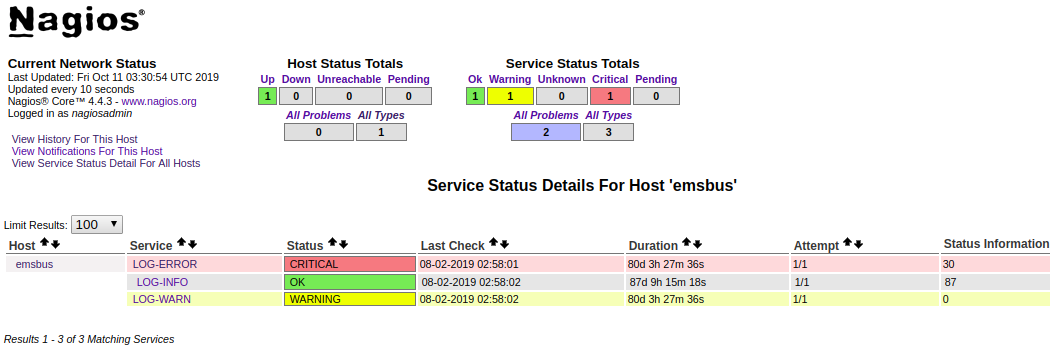
\includegraphics[scale = 0.57]{img/nagiosConfigurado.png}
    \caption{\textit{Dashboard} do Nagios\textsuperscript{\textregistered} com as métricas do registro de \textit{Log}.}
    \label{fun:fig:nagiosDashbordEmsbus}
\end{figure}

\subsubsection{Ems-Monitor}

Neste trabalho, foi realizada uma análise com a ferramenta de monitoramento Observer. Pode-se observar que o Erlangms sem a execução do módulo monitoramento, funciona entre cinco e dez porcento de utilização do \textit{Scheduler}, cinquenta \textbf{MB} de utilização de Memória e com picos de quatrocentos \textbf{B} de utilização de IO. Essa verificação é realizada em tempo real, e pode ser observada na figura \ref{fun:fig:Observer_ErlangMS_sem_SNMP}.

\begin{figure}[H]
    \centering
    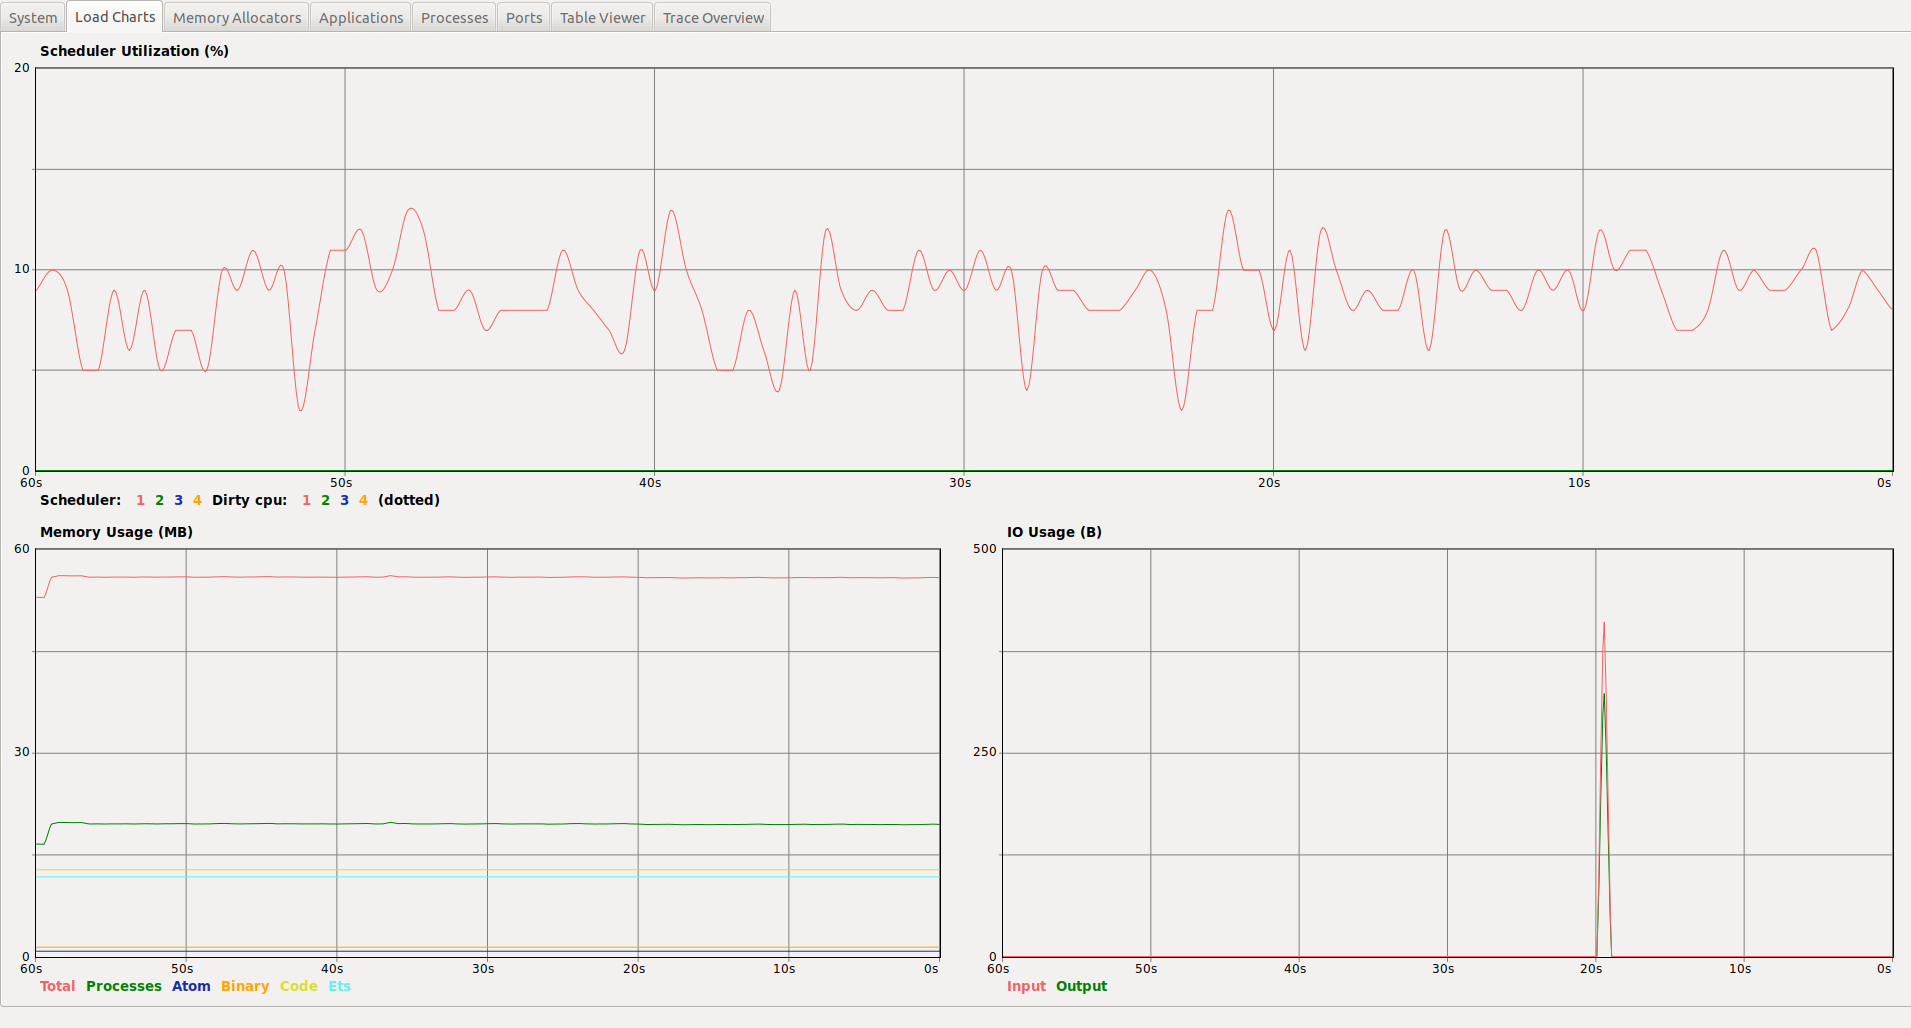
\includegraphics[scale = 0.33]{img/Observer_ErlangMS_sem_SNMP.png}
    \caption{Análise executada em tempo real pela ferramenta Observer.}
    \label{fun:fig:Observer_ErlangMS_sem_SNMP}
\end{figure}

Com a utilização do Ems-monitor ativado no Erlangms, foi possível verificar durante a realização da análise a identificação de \textit{overhead}, no \textit{Scheduler}, Memória e IO. No funcionamento do Ems-monitor o aumento da utilização apresentou as seguintes informações:  o \textit{Scheduler} funcionando entre cinco e quinze porcento de utilização, sessenta \textbf{MB} de utilização de Memória e com aumento na intermitência que variam de vinte \textbf{KB} até cento e quarenta \textbf{KB} de utilização de IO. A análise realizada na ferramenta Observer, para acompanhar o funcionamento do Ems-Monitor pode ser visualizada na figura \ref{fun:fig:Observer_ErlangMS_com_SNMP}.  

\begin{figure}[H]
    \centering
    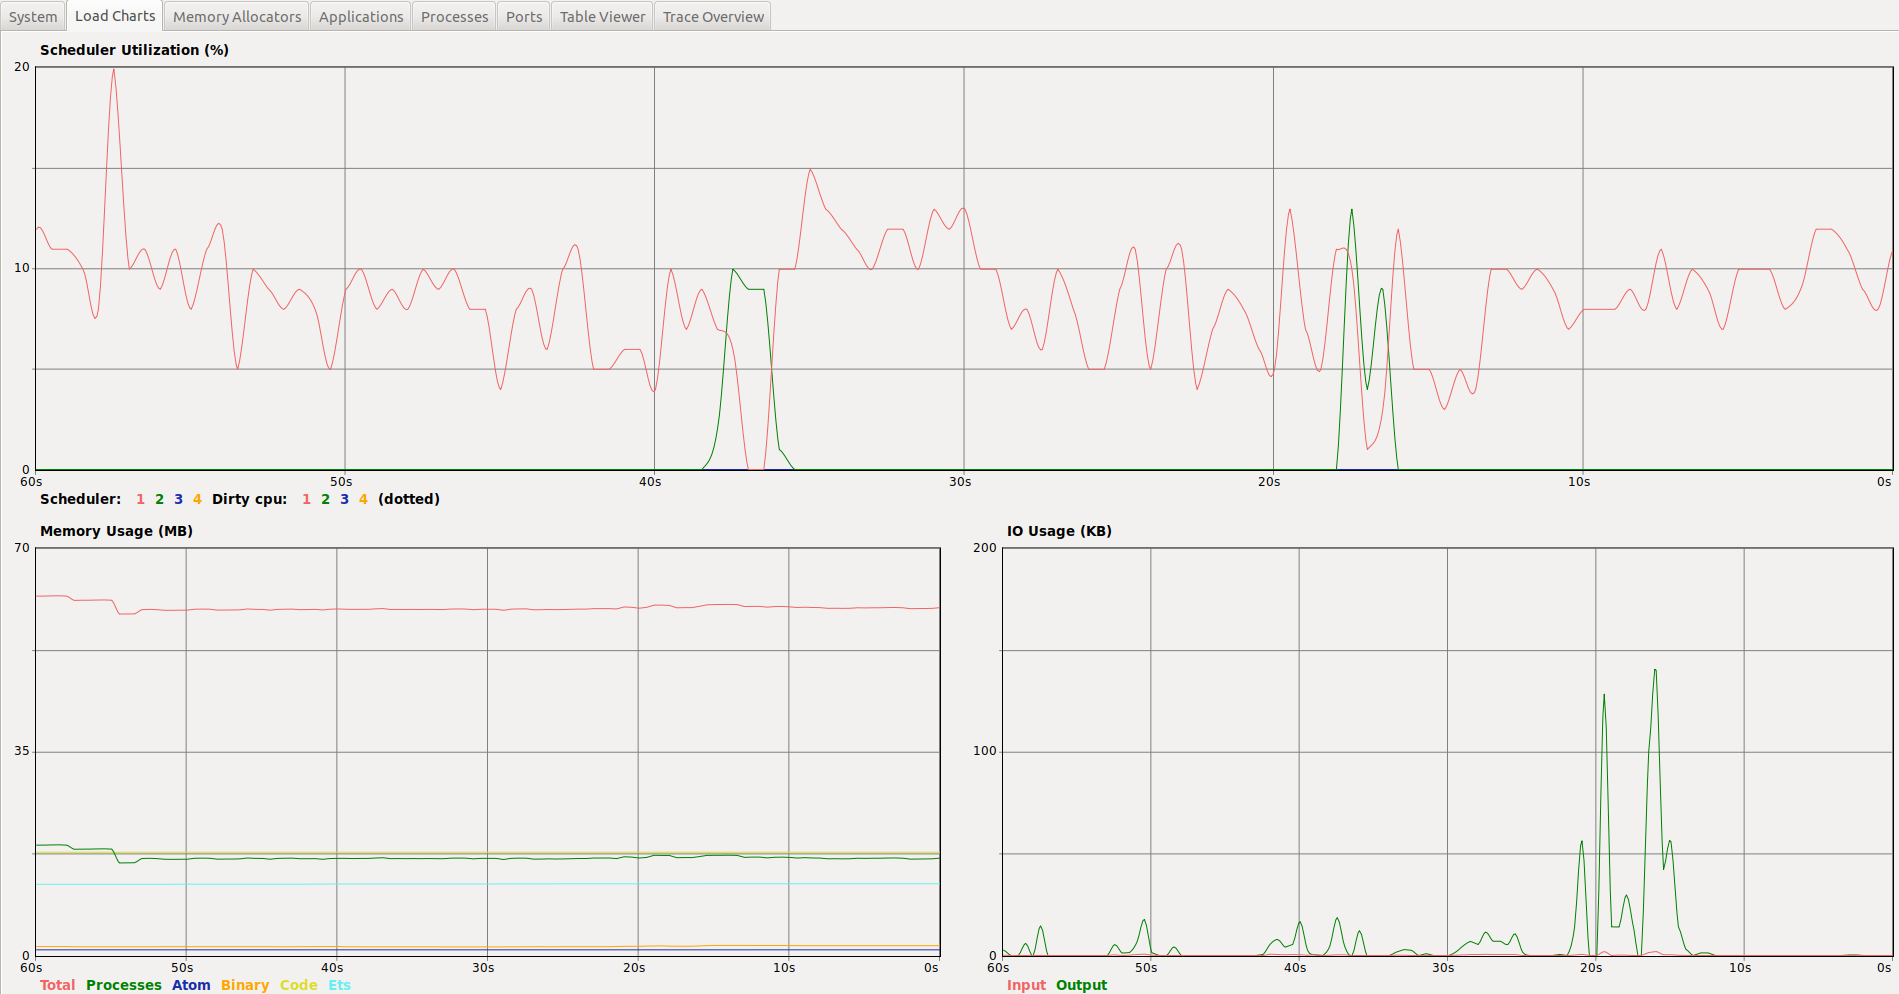
\includegraphics[scale = 0.33]{img/Observer_ErlangMS_com_SNMP.png}
    \caption{Análise executada em tempo real pela ferramenta Observer com o Ems-Monitor.}
    \label{fun:fig:Observer_ErlangMS_com_SNMP}
\end{figure}

Por fim, pode-se observar o aumento da utilização dos recuros computacionais. O \textit{Scheduler} precisou gerenciar mais processos, com o aumento de processos foi necessária a utilização de mais memória, que devido ao funcionamento em modo passivo do Ems-Monitor para o envio de \textit{TRAPs}, teve também aumento IO, pois mesmo sem o funcionamento e execução dos recursos do Erlangms, mensagens são enviadas. O \textit{overhead} gerado pelo funcionamento do Ems-Monitor não demonstrou comprometer de forma impeditiva o funcionamento do Erlangms.    
 
%%%%%%%%%%%%%%%%%%%%%%%%%%%%%%%%%%%%%%%%%%%%%%%%%%%%%%%%%%%%%%%

\section{Síntese do Capítulo}
\label{sintese5}

Este capítulo apresentou a avaliação da aplicações integrantes da execução do monitoramento dos recursos do barramento, a partir dessa avaliação foi possível responder com fundamentação obtida dos resultados que a solução está adequada ao ambiente computacional do \acrshort{CPD} da \acrshort{UnB}, permitindo a possibilidade de implantação após validação pelo colaboradores desse Centro, e disponibilização da próxima versão disponível,para uso exclusivo do barramento de serviços Erlangms.